
% Many thanks to Andrew West for writing most of this file
% Main LaTeX file for CIS400/401 Project Proposal Specification
%
% Once built and in PDF form this document outlines the format of a
% project proposal. However, in raw (.tex) form, we also try to
% comment on some basic LaTeX technique. This is not intended to be a
% LaTeX tutorial, instead just (1) a use-case thereof, and (2) a
% template for your own writing.

% Ordinarily we'd begin by specifying some broad document properties
% like font-size, page-size, margins, etc. -- We have done this (and
% much more) for you by creating a 'style file', which the
% 'documentclass' command references.
\documentclass{sig-alternate}
 
% These 'usepackage' commands are a way of importing additional LaTeX
% styles and formattings that aren't part of the 'standard library'
\usepackage{mdwlist}
\usepackage{url}

\begin{document} 

% We setup the parameters to our title header before 'making' it. Note
% that your proposals should have actual titles, not the generic one
% we have here.
\title{Programming Language Support for Probabilistic Associative Memory}
\subtitle{Dept. of CIS - Senior Design 2014-2015\thanks{Advisor: Steve A. Zdancewic (stevez@cis.upenn.edu).}}
%\thanks{ Do not list your advisors amongst the authors as that may cause Google Scholar to add this work to their list of publications. Your advisor must also sign a hard-copy of your proposal.}}
%\thanks{ }}
\numberofauthors{3}
\author{
    Fan Yin \\ \email{fanyin@seas.upenn.edu}
    \and Haolin Lu \\ \email{haolinlu@seas.upenn.edu}
    \and Yukuan Zhang\\ \email{yukuan@seas.upenn.edu}
}
%\author{
%\alignauthor Radoslav Ivanov \\ \email{rivanov@seas.upenn.edu} \\ Univ. of Pennsylvania \\ Philadelphia, PA 
%
%\and Radoslav Ivanov \\ \email{rivanov@seas.upenn.edu} \\ Univ. of Pennsylvania \\ Philadelphia, PA 
%
%}
\date{}
\maketitle

% Next we write out our abstract -- generally a two paragraph maximum,
% executive summary of the motivation and contributions of the work.
\begin{abstract}
    Our goal is to create a library (OPaml) that provides an interface and implementation 
    for programming with a probablistic associative memory. 
    
    An associative memory allows queries by content rather than by address or location.
    In addition, as with standard memory, associative memory remembers every value stored.

    On the other hand, probabilistic associative memory returns a value based on a probability model 
    for a given memory query. This allows it to use less space than regular
    associative memories, making it useful for applications that prioritize low memory footprints over 
    fidelity. 
%  \textit{The purpose of this document is three-fold. First, it
%    describes the requirements of the project proposal. Second, it
%    presents this information in a style your proposal should
%    mimic. Third, by viewing the *.tex `code behind', some basic
%    \LaTeX{} technique can be learned. Do not feel compelled to
%    completely follow our style -- but do use it as a guide.}%
    
  %\textit{Like this `report', your proposal is expected to have an
  %  abstract. An abstract is a two-paragraph maximum executive summary
  %  of your work. It should briefly outline your problem statement and
  %  its (expected) contributions.}
\end{abstract}

% Then we proceed into the body of the report itself. The effect of
% the 'section' command is obvious, but also notice 'label'. Its good
% practice to label every (sub)-section, graph, equation etc. -- this
% gives us a way to dynamically reference it later in the text via the
% 'ref' command, e.g., instead of writing `Section 1', you can write
% `Section~\ref{sec:intro}', which is useful if the section number
% changes.
\section{Introduction}
\label{sec:intro}

The standard way to access a stored value in memory is by address. 
This involves finding the physical position of that address in memory
and returning the stored value. Associative memory allows
searching for a values based on the stored content. An analagous structure
in programming languages is the hashtable, which returns an output value
based on an input key. 

Associative memories are useful for when one needs to query memory based 
on some input data or tag. For instance, router firmware will often employ associative 
memories to store tables of IP addresses, which serve as the "next hop" for incoming 
packets. Since routers looking for the "next hop" have a specific, standard query 
format -- e.g. an IP address of the form www.xxx.yyy.zzz -- it makes sense to store the 
routing tables based around this input string.

With proabilistic memories, for a given query, we return the most "likely" candidate 
based on some specified probability model of the values stored in memory. 
Since our queries work directly with a probability model, it would offer more fluidity
with programming that involves statistical modeling or simulations. Returning values
based on a probability also saves memory because not every value has to be stored. The 
memory mechanism can extrapolate or interpolate a response to a query based on values 
previously inserted into memory. 

We also strive to add support for structured data in our probabilistic associative memory.
In a standard associative memory scheme, a similarity query is done by comparing input bits
to the values stored in memory. However, this does not allow for good similarity comparisons
between trees or lists, as the memory is not aware of the underlying structure. As a result,
many applications on structured data will first flatten the structure, do the calculations
it needs, then reconstruct the original structure of that data. With a built-in type system
that supports structured data, the user will be able to directly manipulate the data in memory 
while keeping the structure intact.

%You should begin by introducing your topic. You should define core
%terminology specific to the field, introduce the problem statement,
%and make clear the benefits (motivate!) of resolving that problem
%statement. If there are many preliminaries (\textit{e.g.,}
%definitions, conceptual explanations) you need to handle before
%jumping into your topic, it may be worthwhile to create an explicit
%``Background'' section.
%
%Let us suppose you are attempting to build a constant time integer
%factorization algorithm. You would want to briefly explain that
%factorization is the process of breaking an integer into its prime
%multipliers. Give a simple example. Your problem statement would
%conclude that factorization is an unneccesarily complex
%process. Finally, you would state that via your proposed system,
%factorization will be easy and the consequences that will
%have. Namely, the RSA-encryption algorithm will be broken.

% The header of this document might have been a little intimidatating
% to beginners. Notice once you are in the body of the document,
% however, LaTeX commands are minimal and 'normal text' is frequent.
\section{Related Work}
\label{sec:related_work}
Perhaps the most important section of your proposal is \textit{related
  work}. Here you demonstrate that you have read and understand what
others in the field have done. This ensures you (1) know the
state-of-the-art, (2) are not re-doing others work, and (3) you know
the performance levels you must achieve to make a contribution. As you
discuss each related work, make note of how each has advanced the
field. Keep in mind that this section should not read like a regular
research paper you write for other classes. In other words, you should
not just discuss related work for the sake of having a related work
section; rather, tell a story about the state-of-the-art of the field
and where your work fits in.

% Here we see our first citations. It's just a simple command, the
% body of which is the keyword-label assigned to resources over in the
% *.bib file
This section should have in-line citations to your bibliography
(really all sections should have citations, but we expect them to be
most dense in this section). We are going to require that your
proposal has at least $6$ references. Fortunately, \LaTeX{} makes
citations easy. Your TA has had no difficulty, as the work of Ivanov
\textit{et al.}~\cite{ivanov14} demonstrates. Need help with \LaTeX{}?
Be sure to check out~\cite{latex_wikibook} and~\cite{ctan_pdf}, two
helpful on-line resources.

What defines a good resource? Wikipedia is \textbf{NOT} a good
resource. We would like to see references from academic
journals/conferences (ACM, IEEE, etc.). We realize not everyone is
doing pure research and for students with `implementation' projects
such sources may be rare. No matter the case, your sources need to be
reputable.

Let us return to your factorization proposal. You should put out the
earliest related work; na\"{i}ve methods like trial divison and the
Sieve of Eratosthenes, but state they are of no modern relevance. Then
discuss modern methods like the Quadratic Sieve and General Number
Field Sieve. Note the humongous time and memory bounds of these
algorithms. But wait! You are going to propose a better way $\ldots$

\section{Project Proposal}
\label{sec:project_proposal}
We will be using the OCaml language to implement the aforementioned probabilistic 
associative memory. OCaml is a functional language with a strong and versatile type 
system, which will be useful in implementing typed, structured data in our library. 
Based on the specific probability distribution and model in use, our library would return 
a different memory value. As such, our library will have "plug and play" support for 
different probability paradigms. After we have finished creating our library, we will 
write a programs with the library to demonstrate the benefits of using probabilistic 
associative memory. 

%Now is the time to introduce your proposed project in all of its
%glory. Admittedly, this is not the easiest since you probably have not
%done much actual research yet. Even so, setting and realizing
%realistic research goals is an important skill. Begin by summarizing
%what you are going to do and the expected benefit it will bring.

\subsection{Anticipated Approach}
\label{subsec:approach}
Our first step is to create a programming language interface for probabilistic
associative memories. This involves defining a type system as well as a syntax
for programming with an underlying memory. A major component of this syntax will be 
the way to store into a memory, and the different types of queries we can make
to the memory.

Next, we will implement various types of probablistic associative memories.
One implementation would focus on accuracy, and keep track of every value that
was stored in it. Another implementation will try to conserve memory space,
and compress the stored values. We will work on several different compression methods,
including neural networks and network flow equilibrium. Finally we will create
a type of memory to work specifically with structured data, allowing similarity
queries on data types such as lists or trees.

By creating this interface, users of this programming language will be able to
choose the type of memory that most suits the needs of their particular
application. 

%Having summarized \textit{what} you are going to do, its time to
%describe \textit{how} you plan to do it. Our factorization example
%does not work so well here (it is likely impossible to realize) -- so
%let us suppose you are going to create a service that takes a
%cell-phone picture of a building and returns via text-message, the
%name of that building\footnote{Do not use this idea -- someone did it
%  in a previous year.}.
%
%In this case you might want to talk about establishing a server to
%receive pictures via MMS. Once the picture is received, you will run
%an edge extraction algorithm over it. Then, similarity between the
%submitted picture and those stored (and tagged) in a MySQL database
%will be computing using algorithm $XYZ$. Finally, the tag of the most
%similar image will be returned to the user. Do not bore the reader
%with trivial details, but give them an overview; a block-flow diagram
%would prove helpful (and is required).

\subsection{Technical Challenges}
\label{subsec:tech_challenges}
The foremost technical challenge in our project deals with the logistics of incorporating
a probabilistic model into our memory mechanism, the mathematics involved in said models,
and the programming interface exposed to the end user. \textbf{elaborate}

Another challenge involves testing our library and iterating. We must have some  
baseline "fidelity" or "accuracy" per query, and we must make sure that our probabilistic
queries actually process our sample space accurately and return the "smartest" value.


%In this subsection note where you anticipate having \underline{novel}
%difficulty. Maybe you have never setup a MySQL database or even used
%SQL before at all -- yes, that is a challenge -- but not one readers
%care about. More novel would be the fact that many buildings on Penn's
%campus look similar and your classifier may be inaccurate in such
%instances. The purpose of this section is two-fold: 1) you will think
%about which parts of your project would require the most time and
%effort and 2) you will convince the reader that this is a project
%worth undertaking.

\subsection{Evaluation Criteria}
\label{subsec:eval_criteria}
Suppose you have implemented your approach and it is functioning. Now
how are you going to convince readers your approach is better than
what exists? In the factorization example, you could just compare
run-times between algorithms run on the same input. The image
recognition example might use a percentage of accurate
classifications. Other fields may have established testing benchmarks.

No matter the case, you need to prove you have contributed to the
field. This will be easier for some than others. In particular, those
with `sensory' projects involving visual or sonic elements need to
think this point through -- objective measures are always better than
subjective ones.

\section{Research Timeline}
\label{sec:research_timeline}
Finally, we would like you to speculate about the pace of your
research progress. This section need not be lengthy, we would just
like you to specify some milestones so we can gauge your progress
during our intermediate interviews. Let us follow through with our
image recognition example:

% The 'itemize' environment shown here, and its friend 'enumerate'
% (shown below), are used to create indented\bulleted\outline style
% lists.
\begin{itemize*}
	\item {\sc already completed}: Preliminary reading. Began implementation of image-recognition algorithm.\vspace{3pt}
	\item {\sc prior-to thanksgiving} : Photograph buildings for DB. Make algorithm more efficient, tune parameters.\vspace{3pt}
	\item {\sc prior-to christmas} : Create server-MMS interface. Expand tagged DB collection.\vspace{3pt}
	\item {\sc completion tasks} : Verify implementation is bug-free. Conduct accuracy testing. Complete write-up.\vspace{3pt}
	\item {\sc if there's time} : Investigate image pre-processing techniques to improve accuracy.
\end{itemize*}

% We next move onto the bibliography.
\bibliographystyle{plain} % Please do not change the bib-style
\bibliography{prop_spec}  % Just the *.BIB filename

% Here is a dirty hack. We insert so much vertical space that the
% appendices, which want to begin in the left colunm underneath
% "references", are pushed over to the right-hand column. If we looked
% hard enough, there is probably a command to do exactly this (and
% wouldn't need tweaked after edits).
\vspace{175pt}

% We then use appendices to share some additional information with
% you, though you won't need appendices in your own proposal.
\appendix
\section{Other Specifics}
\label{app:other_specifics}
Your proposal need not have appendices like this section and the next
but we still have info to share:

% The usage of 'enumerate' (similar to 'itemize') we talked about
% above

% You may also notice we have many 'vspace' commands lying
% around. These create 'vertical space' and are a way to force LaTeX
% to cooperate, sometimes. Don't get too involved with using them
% initially, though, because adding or deleting a single line of task
% can dramatically change how LaTeX chooses to format, page, and space
% the document
\begin{enumerate*}
\item {\sc proposal length}: We require that your proposal be 4--5
  pages in length, bibliography included. Be careful, \LaTeX{} and our
  style-file in particular are \textit{extremely} space efficient. An
  9-page MS-Word document could easily become a 5-page \LaTeX{}
  one.\vspace{5pt}

\item {\sc plagarism}: \textbf{DO NOT} plagarize. If you are caught,
  you will fail the class (\textit{i.e.}, not graduate), or worse.

\end{enumerate*}

\section{\LaTeX{} Examples}
\label{app:latex_examples}

% This paragraph makes use of dynamic references. Remember how we've
% been 'label'-ing everything; sections, etc? Using 'ref' we can
% reference them. Add a new figure/section at the beginning? This
% technique automatically re-numbers when you build, so you don't have
% to make static changes.
At this point, the proposal specification is complete. From here on
out, we are just going to show off some commonly used \LaTeX{}
technique. Be sure to look at the `code behind' and see
Tab.~\ref{tab:some_table}, Eqn.~\ref{eqn:some_equation} and
Fig.~\ref{fig:some_graph} for the output! Keep in mind that the
appendix is usually not a good place for your figures. Place them
where you need them and remember to refer to them in the body of your
text; otherwise, the reader will keep reading and will miss them!

% Math is obviously one of LaTeX's strengths. Math can be typeset
% in-line, or off-set in equation 'environments' like this. You'll
% need to look up symbols on an as-needed basis, but I'll assure you
% -- they are ALL there.
\begin{equation}
M(p) = \int^\infty_0 (1+\alpha x)^{-\gamma}x^{p-1}dx
\label{eqn:some_equation}
\end{equation}

% We next encounter tables and figures (images). Big things like these
% are known as 'floats' in LaTeX because their position is not
% fixed. Notice that '[htb!]' follows the start of each
% environment. We are telling LaTeX that we'd like to put the
% table/fig 'h' - HERE, precisely where it follows in the
% narrative. If LaTeX determines it doesn't look good here, 't' tells
% LaTeX we'd like it at the top of this column, and if that doesn't
% work, use 'b', the bottom of the column. Other options are
% available. LaTeX shifts floats around to ensure images don't end up
% on page/column boundaries, which would result in a waste of space
% for text.

% We insert a table into the document. Notice the '| c | c | c |'
% argument provided to the tabular environment. This says we want
% three columns, all with center-alignment, with vertical bars between
% them. In the body of argument, an ampersand '&' separates cells, and
% a double forward-slash '\\' is used to create new lines. Otherwise,
% commands should be self explanatory.
\begin{table}[htb!]
	\begin{center}
  \begin{tabular}{| c | c | c |}
    \hline
    \textbf{User Type} & \textbf{Cleanup\%} & \textbf{Honesty\%} \\ \hline
    Good & 90-100\% & 100\% \\ \hline
    Purely Malicous & 0-10\% & 0\% \\ \hline
		Malicious Provider & 0-10\% & 100\% \\ \hline
		Feedback Malicous & 90-100\% & 0\% \\ \hline
		Disguised Malicous & 50-100\% & 50-100\% \\ \hline
		Sybil Attacker & 0-10\% & Irrelevant \\ \hline
  \end{tabular}
	\caption{Example Table}
  \label{tab:some_table}
	\vspace{-10pt}
	\end{center}
\end{table}

% We insert a graph/figure into the document. This is a pretty
% straightforward process once you get the image into a file format
% that LaTeX plays nice with. Then we just scale it as
% a % of the column width.
\begin{figure}[htb!]
	\begin{center}
		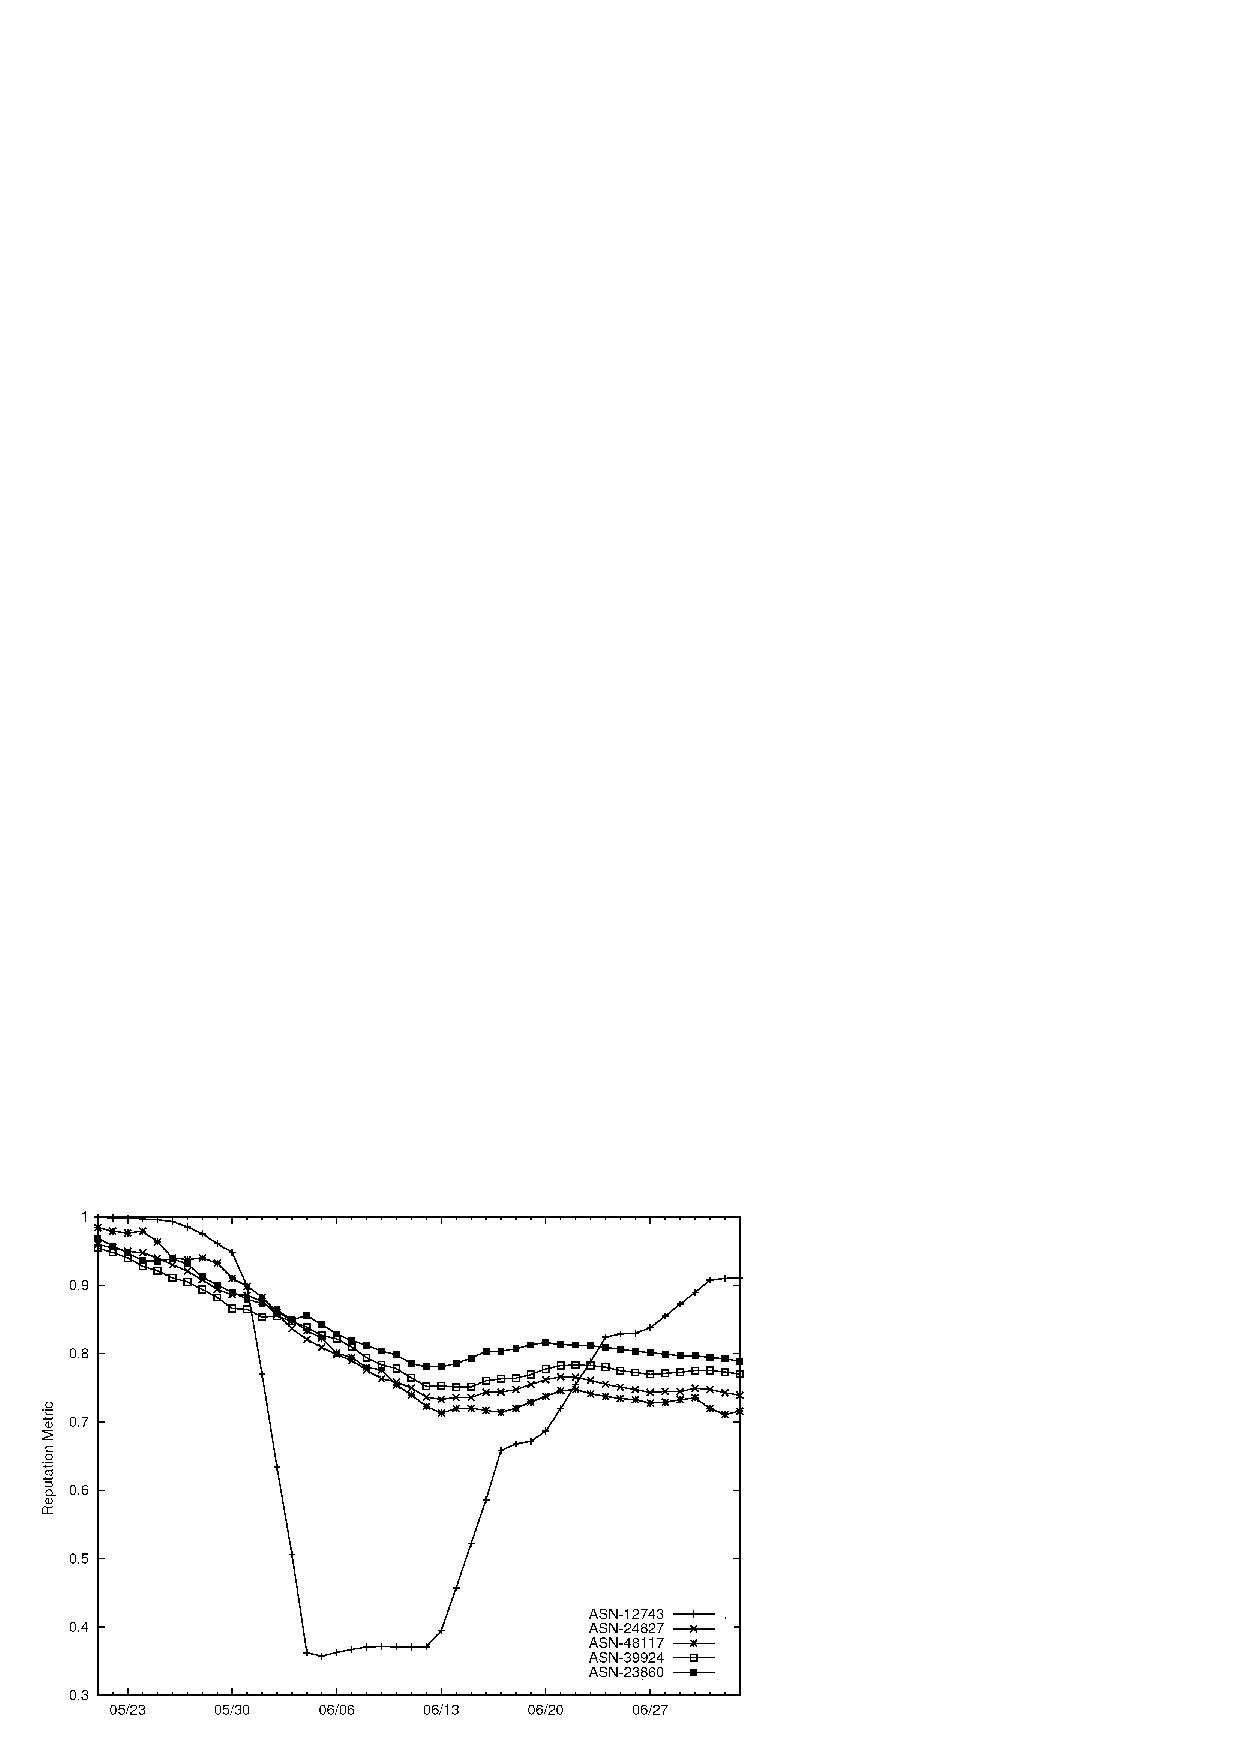
\includegraphics[width=0.75\linewidth]{some_graph}
	\end{center}
	\vspace{-12pt}
	\caption{Example Figure/Graph}
	\label{fig:some_graph}
\end{figure}

\end{document} 

